% ==============================================================================
% Chapter 5: Integrated Hedging Analysis & Derivative Efficiency
% ==============================================================================

\chapter{Integrated Hedging Analysis}
\label{ch:hedging}

\section{Unifying Downside Risk Measurement with Derivative Protection}
\label{sec:unifying_risk_hedging}

In Chapter~\ref{ch:var_modeling}, we established that an institutional shareholder holding \textbf{1 standard NSE market lot} ($1,725$ shares at $S_0 = \text{\rupee}285.00$, with total capital commitment $V_0 = \text{\rupee}4,91,625.00$) faces a severe 10-day $99\%$ Historical Simulation Value at Risk:
\begin{equation}
\VaR_{\text{hist}, 99\%}^{10\text{d}} = \text{\textbf{\rupee 61,487.02}} \quad (12.51\% \text{ of portfolio capital})
\end{equation}
This tail loss quantile implies that over a 10-day market disruption, the equity price of ITC can drop to:
\begin{equation}
S_{T, \VaR} = S_0 \times \left(1 - \VaR_{\text{hist}, 99\%}^{10\text{d}}\right) = 285.00 \times (1 - 0.125069) = \text{\textbf{\rupee 249.36 per share}}
\end{equation}

Rather than accepting this unhedged catastrophic tail exposure, the portfolio manager can deploy non-linear derivative instruments to construct an asymmetric payoff floor. In this chapter, we evaluate the comparative hedging efficiency of three alternative derivative structures:
\begin{enumerate}
    \item \textbf{At-The-Money (ATM) Protective Put:} Long 1 lot Stock + Long 1 lot \rupee 285 Put.
    \item \textbf{Out-of-The-Money (OTM) Protective Put:} Long 1 lot Stock + Long 1 lot \rupee 280 Put.
    \item \textbf{Zero-Cost Collar Strategy:} Long 1 lot Stock + Long 1 lot \rupee 280 Put $-$ Short 1 lot \rupee 295 Call.
\end{enumerate}

\section{Protective Put Payoff Architecture: ATM vs. OTM Insurance}
\label{sec:protective_put_mechanics}

A Protective Put combines a long physical equity position with a long European put option contract. Let $K$ denote the strike price and $P(K)$ denote the upfront option premium paid per share. At expiry $T$, the net terminal profit or loss per share is formulated as:
\begin{align}
\Pi_{\text{prot}}(S_T) &= (S_T - S_0) + \max(K - S_T, 0) - P(K) \label{eq:prot_put_pl} \\
&= \begin{cases}
(K - S_0) - P(K), & \text{if } S_T < K \quad \text{(Protected Floor)} \\
(S_T - S_0) - P(K), & \text{if } S_T \ge K \quad \text{(Full Upside Participation)}
\end{cases}
\end{align}

\subsection{Strategy 1: ATM Protective Put ($K = \text{\rupee}285.00$)}

Using the calibrated December 2026 contract price ($P_{\text{ATM}} = \text{\rupee}8.86$ per share):
\begin{itemize}
    \item \textbf{Total Insurance Cost:} $1,725 \times \text{\rupee}8.86 = \text{\textbf{\rupee 15,283.50}}$.
    \item \textbf{Downside Floor:} For any terminal spot price $S_T < \text{\rupee}285.00$, the put option guarantees the right to sell at \rupee 285.00. Consequently, the equity loss is exactly zero, and the net portfolio loss is \textbf{strictly capped at the upfront premium paid}:
    \begin{equation}
    \mathcal{L}_{\max} = 1,725 \times \text{\rupee}8.86 = \text{\rupee 15,283.50}
    \end{equation}
    \item \textbf{Breakeven Price at Expiry:} $S_0 + P_{\text{ATM}} = 285.00 + 8.86 = \text{\rupee 293.86}$ ($+3.11\%$ above spot).
    \item \textbf{Tail Risk Mitigation at the $99\%$ 10-day $\VaR$ Horizon ($S_T = \text{\rupee}249.36$):} Whereas the unhedged portfolio suffers a loss of \rupee 61,487.02, the ATM protected portfolio loses only \rupee 15,283.50, delivering a \textbf{VaR reduction of $75.14\%$}.
\end{itemize}

\subsection{Strategy 2: OTM Protective Put ($K = \text{\rupee}280.00$)}

To reduce the cash drag of purchasing insurance, the investor can purchase an Out-of-The-Money put option at strike $K = \text{\rupee}280.00$ ($P_{\text{OTM}} = \text{\rupee}6.82$ per share):
\begin{itemize}
    \item \textbf{Total Insurance Cost:} $1,725 \times \text{\rupee}6.82 = \text{\textbf{\rupee 11,764.50}}$ (a cash saving of \rupee 3,519.00 relative to the ATM put).
    \item \textbf{Deductible Exposure:} The investor absorbs the first \rupee 5.00 of equity downside ($S_0 - K = 285 - 280 = \text{\rupee}5.00$). Below \rupee 280, the put absorbs all further losses. The maximum downside loss is:
    \begin{equation}
    \mathcal{L}_{\max} = 1,725 \times \left[(285.00 - 280.00) + 6.82\right] = 1,725 \times \text{\rupee}11.82 = \text{\textbf{\rupee 20,389.50}}
    \end{equation}
    \item \textbf{Breakeven Price at Expiry:} $S_0 + P_{\text{OTM}} = 285.00 + 6.82 = \text{\rupee 291.82}$ ($+2.39\%$ above spot).
    \item \textbf{Tail Risk Mitigation at $\VaR$ Horizon ($S_T = \text{\rupee}249.36$):} Portfolio loss is capped at \rupee 20,389.50, achieving a \textbf{VaR reduction of $66.84\%$}.
\end{itemize}

\section{The Zero-Cost Collar Strategy}
\label{sec:collar_strategy}

While protective puts provide absolute insurance, institutional portfolio managers often resist paying $2.4\%\text{--}3.1\%$ of portfolio capital in upfront option premiums. The \textbf{Zero-Cost Collar} resolves this hurdle by financing the purchase of a protective put through the simultaneous sale of an out-of-the-money covered call:
\begin{itemize}
    \item \textbf{Long Physical Stock:} 1 lot ($1,725$ shares) at $S_0 = \text{\rupee}285.00$.
    \item \textbf{Long OTM Put Option:} Strike $K_1 = \text{\rupee}280.00$ (cost = \rupee 6.82 per share).
    \item \textbf{Short OTM Call Option:} Strike $K_2 = \text{\rupee}295.00$ (premium received = \rupee 4.32 per share).
\end{itemize}
The net upfront debit per share is:
\begin{equation}
\text{Net Debit} = P(280) - C(295) = 6.82 - 4.32 = \text{\textbf{\rupee 2.50 per share}}
\end{equation}
Total upfront cash outflow across the entire lot is only $1,725 \times \text{\rupee}2.50 = \text{\textbf{\rupee 4,312.50}}$ ($0.88\%$ of portfolio value), representing an approximate zero-cost hedge.

The terminal payoff per share is defined piecewise across three distinct spot price zones:
\begin{equation}
\Pi_{\text{collar}}(S_T) = \begin{cases}
(K_1 - S_0) - [P(K_1) - C(K_2)] = -5.00 - 2.50 = \text{\textbf{-\rupee 7.50}}, & S_T \le 280.00 \\[4pt]
(S_T - S_0) - 2.50 = S_T - 287.50, & 280.00 < S_T < 295.00 \\[4pt]
(K_2 - S_0) - [P(K_1) - C(K_2)] = +10.00 - 2.50 = \text{\textbf{+\rupee 7.50}}, & S_T \ge 295.00
\end{cases}
\label{eq:collar_piecewise}
\end{equation}

\begin{figure}[htbp]
\centering
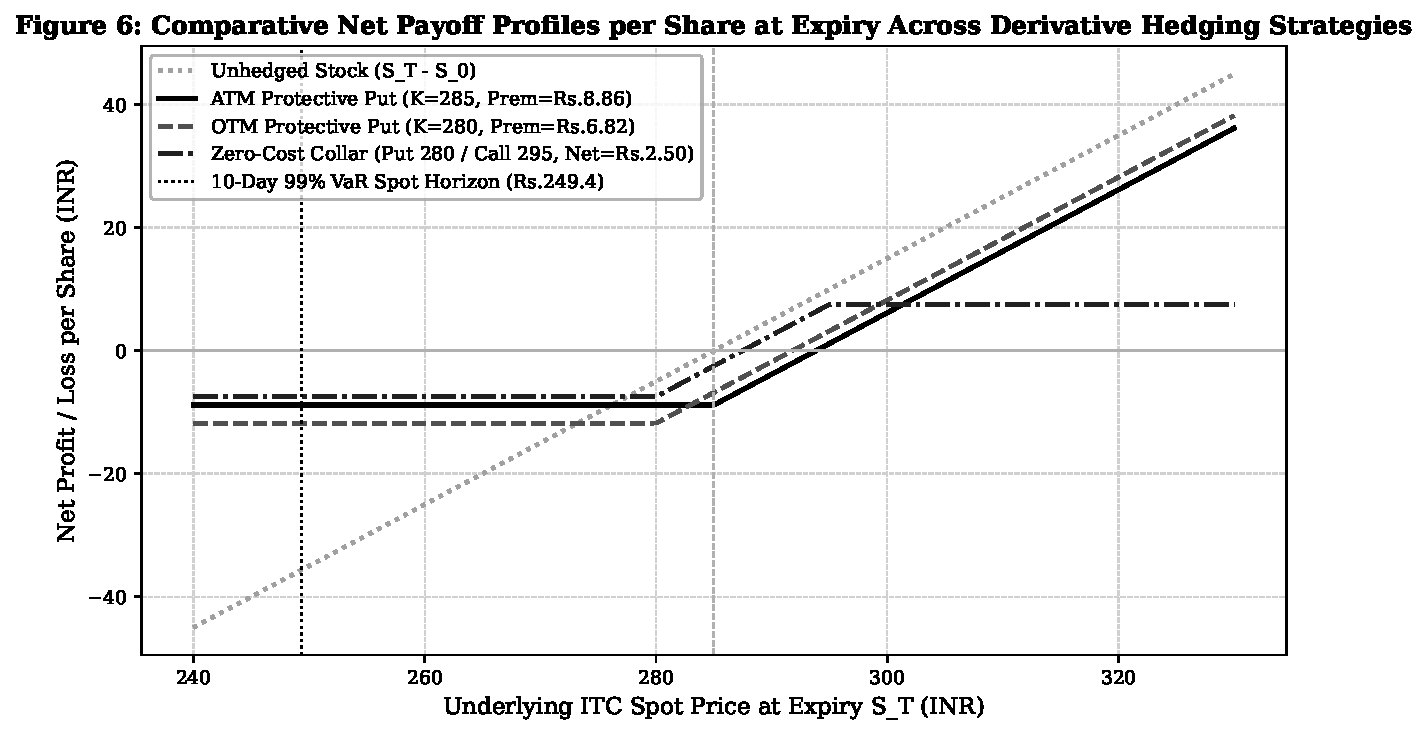
\includegraphics[width=0.96\linewidth]{figures/fig6_hedging_payoffs.pdf}
\caption{Comparative Net Payoff Profiles Across Derivative Hedging Strategies at Expiry}
\label{fig:hedging_payoffs}
\vspace{2pt}
\begin{minipage}{0.96\linewidth}
\footnotesize\textbf{Note:} Expiry profit/loss per share across terminal spot prices $S_T \in [\text{\rupee}240, \text{\rupee}330]$. Plotted strategies: Unhedged Stock (dotted gray), ATM Protective Put (solid black), OTM Protective Put (dashed dark gray), and Zero-Cost Collar (dash-dot black). Vertical dotted line marks the 10-day $99\%$ Historical $\VaR$ horizon ($S_{T, \VaR} = \text{\rupee}249.36$).
\end{minipage}
\end{figure}

\section{Quantitative Hedging Efficiency and Strategy Comparison}
\label{sec:hedging_comparison_matrix}

Table~\ref{tab:hedging_comparison} synthesizes the comparative quantitative risk metrics across all evaluated hedging structures against the unhedged baseline.

\begin{table}[htbp]
\centering
\small
\caption{Comprehensive Derivative Hedging Efficiency Matrix for 1 Lot of ITC ($1,725$ Shares)}
\label{tab:hedging_comparison}
\begin{tabularx}{\linewidth}{Xrrrr}
\toprule
\textbf{Quantitative Metric} & \textbf{Unhedged Stock} & \textbf{ATM Put (285)} & \textbf{OTM Put (280)} & \textbf{Collar (280/295)} \\
\midrule
Position Components & $1,725$ Shares & Stock + Put 285 & Stock + Put 280 & Stock + Put 280 $-$ Call 295 \\
Upfront Cash Cost & \rupee 0.00 & \rupee 15,283.50 & \rupee 11,764.50 & \rupee 4,312.50 \\
Upfront Cost (\% of $V_0$) & $0.00\%$ & $3.11\%$ & $2.39\%$ & $0.88\%$ \\
Breakeven Expiry Price & \rupee 285.00 & \rupee 293.86 & \rupee 291.82 & \rupee 287.50 \\
Max Downside Loss / Share & $-\text{\rupee}285.00$ & $-\text{\rupee}8.86$ & $-\text{\rupee}11.82$ & $-\text{\rupee}7.50$ \\
Total Maximum Loss ($1$ Lot) & $-\text{\rupee}4,91,625.00$ & $-\text{\rupee}15,283.50$ & $-\text{\rupee}20,389.50$ & $-\text{\rupee}12,937.50$ \\
Maximum Upside Potential & Unlimited & Unlimited & Unlimited & $+\text{\rupee}12,937.50$ (Capped at 295) \\
\textbf{Loss at 10d 99\% VaR} & \textbf{-\rupee 61,487.02} & \textbf{-\rupee 15,283.50} & \textbf{-\rupee 20,389.50} & \textbf{-\rupee 12,937.50} \\
\textbf{Tail Risk Reduction (\%)} & \textbf{0.00\%} & \textbf{+75.14\%} & \textbf{+66.84\%} & \textbf{+78.96\%} \\
\bottomrule
\end{tabularx}
\end{table}

\begin{empiricalbox}{Hedging Strategy Synthesis and Optimization}{hedging_synthesis}
As shown in Table~\ref{tab:hedging_comparison} and Figure~\ref{fig:hedging_payoffs}:
\begin{enumerate}
    \item The \textbf{ATM Protective Put} delivers pure insurance, eliminating $75.14\%$ of extreme 10-day downside risk while preserving unlimited upside participation, at an insurance cost of $3.11\%$ of capital.
    \item The \textbf{Zero-Cost Collar} achieves the highest tail risk reduction (\textbf{+78.96\%}), cutting capital loss at the $99\%$ $\VaR$ horizon from \rupee 61,487.02 down to \rupee 12,937.50. This is achieved at a negligible cash outlay of \rupee 4,312.50, by agreeing to surrender equity gains beyond \rupee 295.00 ($+3.51\%$ above spot).
\end{enumerate}
For an institutional asset manager benchmarked to dividend yield and downside preservation, the Collar provides the most cost-efficient risk-adjusted hedge.
\end{empiricalbox}

\section{Dynamic Delta-Hedging vs. Static Insurance Considerations}
\label{sec:dynamic_delta_hedging}

Rather than maintaining a static option contract until expiry, quantitative desks frequently deploy \textbf{Dynamic Delta-Hedging} to neutralize directional market exposure:
\begin{equation}
\Delta_{\Pi} = \Delta_{\text{stock}} + n_c \cdot \Delta_{\text{call}} + n_p \cdot \Delta_{\text{put}} = 0
\end{equation}
However, dynamic delta replication faces severe real-world frictions in the Indian F\&O market:
\begin{itemize}
    \item \textbf{Gamma Risk and Continuous Rebalancing:} As demonstrated in Figure~\ref{fig:option_greeks} (Panel B), Gamma peaks at the ATM strike ($\Gamma = 0.0175$). As spot fluctuates, Delta shifts rapidly ($\dd \Delta \approx \Gamma \dd S$), requiring continuous intraday stock rebalancing.
    \item \textbf{Transaction Costs and Securities Transaction Tax (STT):} In India, high STT on cash equity and derivative turnover, combined with bid-ask spreads on the NSE order book, creates a cumulative rebalancing drag that frequently exceeds the theoretical option premium of a static protective put.
    \item \textbf{Discrete Market Jumps:} When major regulatory policy announcements or Union Budget tobacco taxes occur overnight, equity prices gap down discontinuously, bypassing continuous delta stops and triggering catastrophic replication slippage.
\end{itemize}
Consequently, static option hedges (Protective Puts and Collars) provide vastly superior protection against discrete gap risk compared to dynamic delta replication.
